\providecommand{\main}{..}
\documentclass[\main/notes.tex]{subfiles}

\begin{document}
	\setcounter{chapter}{2}
	\chapter{Vectors in 2-Space and 3-Space}
		\section{Introduction to Vectors}
			\begin{definition}{Vector}
				A quantity with both magnitude and direction. Can be written in bold, for example, $\mathbf{v}$, or as $\overrightarrow{v}$.

				A vector that has an initial point $A$ and terminal point $B$ is written:
				\begin{align*}
					\overrightarrow{v} = \overrightarrow{AB}
				\end{align*}

				Vectors with the same length and direction are said to be \concept{equivalent}.
			\end{definition}
			\begin{sidenote}{Vectors whose initial point is not at the origin}
				If $\overrightarrow{P_{1}P_{2}}$ denotes the vector with initial point $P_{1}(x_{1}, y_{1}, z_{1})$ and terminal point $P_{2}(x_{2}, y_{2}, z_{2})$, then the components of the vector are:
				\begin{align*}
					\overrightarrow{P_{1}P_{2}} = \left\langle x_{2} - x_{1}, y_{2} - y_{1}, z_{2} - z_{1}\right\rangle
				\end{align*}
			\end{sidenote}
			\begin{sidenote}{Vector Algebraic Operations}
				If $\mathbf{u}$, $\mathbf{v}$ and $\mathbf{w}$ are vectors in $\mathbb{R}^{n}$, and if $k$ and $m$ are scalars, then:
				\begin{enumerate}[label=(\alph*)]
					\item $\mathbf{u} + \mathbf{v} = \mathbf{v} + \mathbf{u}$
					\item $(\mathbf{u} + \mathbf{v}) + \mathbf{w} = \mathbf{u} + (\mathbf{v} + \mathbf{w})$
					\item $\mathbf{u} + \mathbf{0} = \mathbf{0} + \mathbf{u} = \mathbf{u}$
					\item $\mathbf{u} + (-\mathbf{u}) = \mathbf{0}$
					\item $k(\mathbf{u} + \mathbf{v}) = k\mathbf{u} + kv$
					\item $(k + m)\mathbf{u} = k\mathbf{u} + m\mathbf{u}$
					\item $k(m\mathbf{u}) = km(\mathbf{u})$
				\end{enumerate}
			\end{sidenote}
			\begin{theorem}{Linear Combination}
				If $\mathbf{w}$ is a vector in $\mathbb{R}^{n}$, then $\mathbf{w}$ is called a \concept{linear combination} of the vectors $\mathbf{v_{1}}$, $\mathbf{v_{2}}$, $\ldots$, $\mathbf{v_{r}}$ in $\mathbb{R}^{n}$ if it can be expressed in the form:
				\begin{align*}
					\mathbf{w} = k_{1}\mathbf{v_{1}} + k_{2}\mathbf{v_{2}} + \cdots + k_{r}\mathbf{v_{r}}
				\end{align*}
				where $k_{1}$, $k_{2}$, $k_{r}$ are scalars, called the \concept{coefficients} of the linear combination.
			\end{theorem}

		\section{Norm of a Vector and Distance}
			\begin{definition}{Norm of a Vector}
				If $\mathbf{v} = \left\langle v_{1}, v_{2}, \ldots, v_{n}\right\rangle$ is a vector in $\mathbb{R}^{n}$, then the \concept{norm} of $\mathbf{v}$, also called the \concept{magnitude} or \concept{length} of $\mathbf{v}$, is written $\left\lVert \mathbf{v}\right\rVert$, and is defined by:
				\begin{align*}
					\left\lVert \mathbf{v}\right\rVert = \sqrt{v_{1}^{2} + v_{2}^{2} + \cdots + v_{n}^{2}}
				\end{align*}
			\end{definition}
			\begin{sidenote}{Properties of the Norm}
				If $\mathbf{v}$ is a vector in $\mathbb{R}^{n}$, and $k$ is any scalar, then:
				\begin{enumerate}[label=(\alph*)]
					\item $ \left\lVert \mathbf{v}\right\rVert \geq 0$
					\item $ \left\lVert \mathbf{v}\right\rVert = 0$ iff $\mathbf{v} = \mathbf{0}$
					\item $ \left\lVert k\mathbf{v}\right\rVert = \left\lvert k\right\rvert \cdot \left\lVert \mathbf{v}\right\rVert$
				\end{enumerate}
			\end{sidenote}
			\begin{definition}{Unit Vector}
				A vector with the norm $1$. If $\mathbf{u}$ denotes the unit vector, and $\mathbf{v}$ is some vector, then the unit vector in the same direction can be calculated as:
				\begin{align*}
					\mathbf{u} = \frac{1}{\left\lVert \mathbf{v}\right\rVert} \cdot \mathbf{v}
				\end{align*}
			\end{definition}
			\begin{sidenote}{The standard unit vectors}
				The vectors in the positive direction of the coordinate axes are called \concept{standard unit vectors}. These are denoted as:
				\begin{alignat*}{3}
					\mathbf{i} &= \left\langle 1, 0, 0\right\rangle & \qquad
					\mathbf{j} &= \left\langle 0, 1, 0\right\rangle & \qquad
					\mathbf{k} &= \left\langle 0, 0, 1\right\rangle
				\end{alignat*}
			\end{sidenote}
			\begin{definition}{Distance in $\mathbb{R}^{n}$}
				If $\mathbf{u} = (u_{1}, u_{2}, \ldots, u_{n}) $ and $mathbf{v} = (v_{1}, v_{2}, \ldots, v_{n})$ are points in $\mathbb{R}^{n}$, then the distance between $\mathbf{u}$ and $\mathbf{v}$ is written $d(\mathbf{u}, \mathbf{v})$, and defined to be:
				\begin{align*}
					d(\mathbf{u}, \mathbf{v}) = \left\lVert u - v\right\rVert
					= \sqrt{(u_{1} - v_{1})^{2} + (u_{2} - v_{2})^{2} + \cdots + (u_{n} - v_{n})^{2}}
				\end{align*}
			\end{definition}

		\section{Dot Product}
			\begin{definition}{Dot Product (Angle)}
				If $\mathbf{u}$ and $\mathbf{v}$ are nonzero vectors in $\mathbb{R}^{2}$ or $\mathbb{R}^{3}$, and if $\theta$ is the angle between $\mathbf{u}$ and $\mathbf{v}$, then the \concept{dot product} (also called the \concept{Euclidean inner product}) of $\mathbf{u}$ and $\mathbf{v}$ is denoted $\mathbf{u} \cdot \mathbf{v}$, and is defined as:
				\begin{align*}
					\mathbf{u} \cdot \mathbf{v} &= \left\lVert \mathbf{u}\right\rVert \left\lVert \mathbf{v}\right\rVert \cos \theta
				\end{align*}
				If $\mathbf{u} = \mathbf{0}$, or $\mathbf{v} = \mathbf{0}$, then $\mathbf{u} \cdot \mathbf{v} = 0$.
			\end{definition}
			\begin{sidenote}{The sign of the dot product and the angle}
				\begin{itemize}
					\item $\theta$ is acute if $\mathbf{u} \cdot \mathbf{v} > 0$
					\item $\theta$ is obtuse if $\mathbf{u} \cdot \mathbf{v} < 0$
					\item $\theta$ is $\pi/2$ if $\mathbf{u} \cdot \mathbf{v} = 0$
				\end{itemize}
			\end{sidenote}
			\begin{definition}{Component form of the dot product}
				The dot product can be represented as the sum of the products of the corresponding components.

				If $\mathbf{u} = \left\langle u_{1}, u_{2}, \ldots, u_{n}\right\rangle$ and $\mathbf{v} = \left\langle v_{1}, v_{2}, \ldots, v_{n}\right\rangle$ are vectors in $\mathbb{R}^{n}$, then the \concept{dot product} is denoted $\mathbf{u} \cdot \mathbf{v}$, and is defined as:
				\begin{align*}
					\mathbf{u} \cdot \mathbf{v} = u_{1}v_{1} + u_{2}v_{2} + \cdots + u_{n}v_{n}
				\end{align*}
			\end{definition}
			\begin{theorem}{Parallelogram Equation for Vectors}
				The sum of the squarea of the diagonals is equal to the sum of the squares of the four sides.

				If $\mathbf{u}$ and $\mathbf{v}$ are vectors in $R^{n}$, then
				\begin{align*}
					\left\lVert \mathbf{u} + \mathbf{v}\right\rVert^{2} + \left\lVert \mathbf{u} - \mathbf{v}\right\rVert^{2} = 2 \biggl(\left\lVert \mathbf{u} \right\rVert^{2} + \left\lVert\mathbf{v}\right\rVert^{2}\biggr)
				\end{align*}
			\end{theorem}
			\begin{theorem}{Dot Product and the Norm}
				If $\mathbf{u}$ and $\mathbf{v}$ are vectors in $\mathbb{R}^{n}$, then
				\begin{align*}
					\mathbf{u} \cdot \mathbf{v} = \frac{1}{4}\left\lVert \mathbf{u} + \mathbf{v}\right\rVert^{2} - \frac{1}{4}\left\lVert \mathbf{u} - \mathbf{v}\right\rVert^{2}
				\end{align*}
			\end{theorem}
			\begin{definition}{Orthogonality}
				Two nonzero vectors $\mathbf{u}$ and $\mathbf{v}$ in $\mathbb{R}^{n}$ are said to be \concept{orthogonal} (or \concept{perpendicular}) if $\mathbf{u} \cdot \mathbf{v} = 0$. The zero vector in $\mathbb{R}^{n}$ is orthogonal to every vector in $\mathbb{R}^{n}$.
			\end{definition}

		\section{Projections}
			\begin{definition}{Orthogonal Projections}
				Decompose a vector $\mathbf{u}$ into a sum of two terms: a scalar multiple of a specified nonzero vector $\mathbf{a}$, and the other term being orthogonal to $\mathbf{a}$.

				If $\mathbf{u}$ and $\mathbf{a}$ are vectors in $\mathbb{R}^{2}$ so that their initial points coincide at a point $Q$, then $\mathbf{u}$ can be decomposed by:
				\begin{enumerate}
					\item Drop a perpendicular from the tip of $\mathbf{u}$ to the line through $\mathbf{a}$.
					\item Construct the vector $\mathbf{w_{1}}$ from $Q$ to the foot of the perpendicular
					\item Construct the vector $\mathbf{w_{2}} = \mathbf{u} - \mathbf{w_{1}}$
				\end{enumerate}
				\begin{center}
					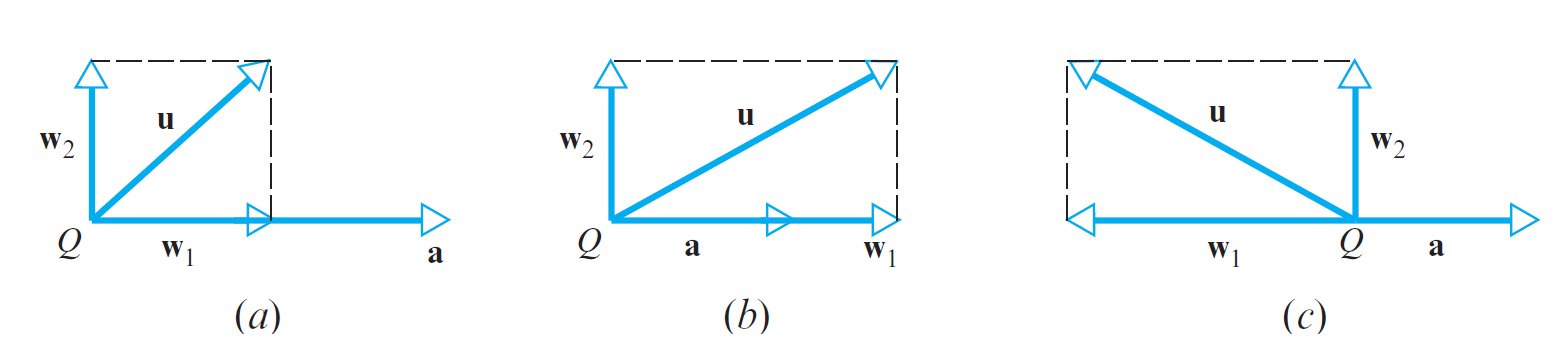
\includegraphics[width=0.85\textwidth]{\main/images/unit03/projection_example.png}
				\end{center}
			\end{definition}
			\begin{theorem}{Projection Theorem}
				If $\mathbf{u}$ and $\mathbf{a}$ are vectors in $\mathbb{R}^{n}$, and if $\mathbf{a} \neq 0$, then $\mathbf{u}$ can be expressed in exactly one way in the form $\mathbf{u} = \mathbf{w_{1}} + \mathbf{w_{2}}$, where $\mathbf{w_{1}}$ is a scalar multiple of $\mathbf{a}$, and $\mathbf{w_{2}}$ is orthogonal to $\mathbf{a}$.
			\end{theorem}
			\begin{definition}{Orthogonal projection of $\mathbf{u}$ on $\mathbf{a}$}
				The vector $\mathbf{w_{1}}$ above is called the \concept{orthogonal projection of $\mathbf{u}$ on $\mathbf{a}$}, or the \concept{vector component of $\mathbf{u}$ along $\mathbf{a}$}. It is commonly written $\proj_{\mathbf{a}}\mathbf{u}$.
				\begin{align*}
					\proj_{\mathbf{a}}\mathbf{u} = \frac{\mathbf{u} \cdot \mathbf{a}}{\left\lVert \mathbf{a}\right\rVert^{2}}\mathbf{a}
				\end{align*}
			\end{definition}
			\begin{definition}{Vector component of $\mathbf{u}$ orthogonal to $\mathbf{a}$}
				The vector $\mathbf{w_{2}}$ above is called the \concept{vector component of $\mathbf{u}$ orthogonal to $\mathbf{a}$}.
				\begin{align*}
					\mathbf{w_{2}} &= \mathbf{u} - \proj_{\mathbf{a}}\mathbf{u}\\
					&= \mathbf{u} - \frac{\mathbf{u} \cdot \mathbf{a}}{\left\lVert \mathbf{a}\right\rVert^{2}}\mathbf{a}
				\end{align*}
			\end{definition}
			\pagebreak
			\begin{definition}{The norm of the orthogonal projection}
				\begin{align*}
					\left\lVert \proj_{\mathbf{a}}\mathbf{u}\right\rVert = \frac{\left\lvert \mathbf{u} \cdot \mathbf{a}\right\rvert }{\left\lVert \mathbf{a}\right\rVert}
				\end{align*}

				In terms of angles, if $\theta$ denotes the angle between $\mathbf{u}$ and $\mathbf{a}$, then $\mathbf{u} \cdot \mathbf{a} = \left\lVert \mathbf{u}\right\rVert \left\lVert \mathbf{a}\right\rVert \left\lvert \cos \theta\right\rvert $.
				So,
				\begin{align*}
					\left\lVert \proj_{\mathbf{a}}\mathbf{u}\right\rVert = \left\lVert \mathbf{u}\right\rVert \cdot \left\lvert \cos \theta\right\rvert 
				\end{align*}
			\end{definition}
			\begin{theorem}{Pythagoras}
				If $\mathbf{u}$ and $\mathbf{v}$ are orthogonal vectors in $\mathbb{R}^{n}$, then:
				\begin{align*}
					\left\lVert \mathbf{u} + \mathbf{v}\right\rVert^{2} = \left\lVert \mathbf{u}\right\rVert^{2} + \left\lVert \mathbf{v}\right\rVert^{2}  
				\end{align*}
			\end{theorem}
			\begin{definition}{Distances Between Points}
				In $\mathbb{R}^{2}$, the distance $D$ between the point $P_{0}(x_{0}, y_{0})$ and the line $ax + by + c = 0$ is:
				\begin{align*}
					D = \frac{\left\lvert ax_{0} + by_{0} + c\right\rvert }{\sqrt{a^{2} + b^{2}}}
				\end{align*}

				In $\mathbb{R}^{3}$, the distance $D$ between the point $P_{0}(x_{0}, y_{0}, z_{0})$ and the plane $ax + by + cz + d = 0$ is:
				\begin{align*}
					D = \frac{\left\lvert ax_{0} + by_{0} + cz_{0} + d\right\rvert }{\sqrt{a^{2} + b^{2} + c^{2}}}
				\end{align*}
			\end{definition}

		\section{Cross Product}
			\begin{definition}{Cross Product}
				If $\mathbf{u} = \left\langle u_{1}, u_{2}, u_{3}\right\rangle$ and $\mathbf{v} = \left\langle v_{1}, v_{2}, v_{3}\right\rangle$ are vectors in $3$-space, then the \concept{cross product} $\mathbf{u} \times \mathbf{v}$ is the \emph{vector} defined by
				\begin{align*}
					\mathbf{u} \times \mathbf{v} = \left\langle u_{2}v_{3} = u_{3}v_{2}, u_{3}v_{1} - u_{1}v_{3}, u_{1}v_{2} - u_{2}v_{1}\right\rangle 
				\end{align*}

				In determinant notation, this can be written:
				\begin{align*}
					\mathbf{u} \times \mathbf{v} = \left( \begin{vmatrix}
						u_{2} & u_{3}\\
						v_{2} & v_{3}
					\end{vmatrix}, - \begin{vmatrix}
						u_{1} & u_{3}\\
						v_{1} & v_{3}
					\end{vmatrix}, \begin{vmatrix}
						u_{1} & u_{2}\\
						v_{1} & v_{2}
					\end{vmatrix}\right)
				\end{align*}

				Using the standard unit vectors, it can also be represented symbolically in the form:
				\begin{align*}
					\mathbf{u} \times \mathbf{v} = \begin{vmatrix}
						\mathbf{i} & \mathbf{j} & \mathbf{k}\\
						u_{1} & u_{2} & u_{3}\\
						v_{1} & v_{2} & v_{3}
					\end{vmatrix}
					= \begin{vmatrix}
						u_{2} & u_{3}\\
						v_{2} & v_{3}
					\end{vmatrix} \mathbf{i} -
					\begin{vmatrix}
						u_{1} & u_{3}\\
						v_{1} & v_{3}
					\end{vmatrix} \mathbf{j} + 
					\begin{vmatrix}
						u_{2} & u_{3}\\
						v_{2} & v_{3}
					\end{vmatrix} \mathbf{k}
				\end{align*}
			\end{definition}
			\begin{sidenote}{Relationships between dot product and cross product}
				If $\mathbf{u}$, $\mathbf{v}$, and $\mathbf{w}$ are vectors in $3$-space, then
				\begin{enumerate}[label=(\alph*)]
					\item $\mathbf{u} \cdot (\mathbf{u} \times \mathbf{v}) = 0$
					\item $\mathbf{v} \cdot (\mathbf{u} \times \mathbf{v}) = 0$
					\item $\left\lVert \mathbf{u} \times \mathbf{v}\right\rVert^{2} = \left\lVert \mathbf{u}\right\rVert^{2}\left\lVert \mathbf{v}\right\rVert^{2} - (\mathbf{u} \cdot \mathbf{v})^{2}$
					\item $\mathbf{u} \times (\mathbf{v} \times \mathbf{w}) = (\mathbf{u} \cdot \mathbf{w})\mathbf{v} - (\mathbf{u} \times \mathbf{v})\mathbf{w}$
					\item $(\mathbf{u} \times \mathbf{v}) \times \mathbf{w} = (\mathbf{u} \cdot \mathbf{w})\mathbf{v} - (\mathbf{v} \times \mathbf{w})\mathbf{u}$
				\end{enumerate}
			\end{sidenote}
			\begin{sidenote}{Properties of the Cross Product}
				If $\mathbf{u}$, $\mathbf{v}$, and $\mathbf{w}$ are vectors in $3$-space, and $k$ is any scalar, then
				\begin{enumerate}[label=(\alph*)]
					\item $\mathbf{u} \times \mathbf{v} = -(\mathbf{v} \times \mathbf{u})$
					\item $\mathbf{u} \times (\mathbf{v} + \mathbf{w}) = (\mathbf{u} \times \mathbf{v}) + (\mathbf{u} \times \mathbf{w})$
					\item $(\mathbf{u} + \mathbf{v}) \times \mathbf{w} = (\mathbf{u} \times \mathbf{w}) + (\mathbf{v} \times \mathbf{w})$
					\item $k(\mathbf{u} \times \mathbf{v}) = (k \mathbf{u}) \times \mathbf{v} = \mathbf{u} \times (k \mathbf{v})$
					\item $\mathbf{u} \times \mathbf{0} = \mathbf{0} \times \mathbf{u} = \mathbf{0}$
					\item $\mathbf{u} \times \mathbf{u} = \mathbf{0}$
				\end{enumerate}
			\end{sidenote}
			\subsection{Geometric Interpretation of the Cross Product}
				\begin{theorem}{Geometric Interpretation of the Cross Product}
					If $\theta$ denotes the angle between two vectors $\mathbf{u}$ and $\mathbf{v}$, then
					\begin{align*}
						\left\lVert \mathbf{u} \times \mathbf{v}\right\rVert = \left\lVert \mathbf{u}\right\rVert \left\lVert \mathbf{v}\right\rVert \sin \theta
					\end{align*}
				\end{theorem}
				\begin{definition}{Area of a Parallelogram}
					If $\mathbf{u}$ and $\mathbf{v}$ are vectors in $3$-space, then $\left\lVert \mathbf{u} \times \mathbf{v}\right\rVert$ is equal to the area of the parallelogram determined by $\mathbf{u}$ and $\mathbf{v}$.
					\begin{align*}
						\Area \square = \left\lVert \mathbf{u} \times \mathbf{v}\right\rVert
					\end{align*}
				\end{definition}
				\begin{definition}{Area of a Triangle}
					If $\mathbf{u}$ and $\mathbf{v}$ are vectors in $3$-space, then the area of the triangle is equal to half the area of the parallelogram.
					\begin{align*}
						\Area \triangle = \frac{1}{2} \left\lVert \mathbf{u} \times \mathbf{v}\right\rVert
					\end{align*}
				\end{definition}
				\begin{definition}{Scalar Triple Product}
					If $\mathbf{u}$, $\mathbf{v}$ and $\mathbf{w}$ are vectors in $3$-space, then
					\begin{align*}
						\mathbf{u} \cdot (\mathbf{v} \times \mathbf{w})
					\end{align*}
					is called the \concept{scalar triple product} of $\mathbf{u}$, $\mathbf{v}$ and $\mathbf{w}$.

					This can be calculated as:
					\begin{align*}
						\mathbf{u} \cdot (\mathbf{v} \times \mathbf{w}) = \begin{vmatrix}
							u_{1} & u_{2} & u_{3}\\
							v_{1} & v_{2} & v_{3}\\
							w_{1} & w_{2} & w_{3}
						\end{vmatrix}
					\end{align*}
				\end{definition}

			\subsection{Geometric Interpretation of Determinants}
				\begin{definition}{Area of the Parallelogram in $2$-space}
					The absolute value of the determinant
					\begin{align*}
						\begin{vmatrix}
							u_{1} & u_{2}\\
							v_{1} & v_{2}
						\end{vmatrix}
					\end{align*}
					is equal to the area of the parallelogram in $2$-space determined by the vectors $\mathbf{u} = \left\langle u_{1}, u_{2}\right\rangle $ and $\mathbf{v} = \left\langle v_{1}, v_{2}\right\rangle $
				\end{definition}
				\begin{definition}{Volume of the Parallelopiped}
					The absolute value of the determinant
					\begin{align*}
						\begin{vmatrix}
							u_{1} & u_{2} & u_{3}\\
							v_{1} & v_{2} & v_{3}\\
							w_{1} & w_{2} & w_{3}
						\end{vmatrix}
					\end{align*}
					is equal to the volume of the parallelopiped in $3$-space determined by the vectors $\mathbf{u} = \left\langle u_{1}, u_{2}, u_{3}\right\rangle $, $\mathbf{v} = \left\langle v_{1}, v_{2}, v_{3}\right\rangle $, and $\mathbf{w} = \left\langle w_{1}, w_{2}, w_{3}\right\rangle $

					This is equal to the absolute of the scalar triple product.
				\end{definition}
				\begin{definition}{Vectors on the same plane}
					If the vectors $\mathbf{u} = \left\langle u_{1}, u_{2}, u_{3}\right\rangle $, $\mathbf{v} = \left\langle v_{1}, v_{2}, v_{3}\right\rangle $, and $\mathbf{w} = \left\langle w_{1}, w_{2}, w_{3}\right\rangle $ have the same initial point, then they lie on the same plane iff
					\begin{align*}
						\mathbf{u} \cdot (\mathbf{v} \times \mathbf{w}) = \begin{vmatrix}
							u_{1} & u_{2} & u_{3}\\
							v_{1} & v_{2} & v_{3}\\
							w_{1} & w_{2} & w_{3}
						\end{vmatrix} = 0
					\end{align*}
				\end{definition}
		\pagebreak

		\section{Lines and Planes in 3-Space}
			\subsection{Point Normal Equations}
				\begin{itemize}
					\item A line is uniquely defined by its slope, and one of its points.
					\item A plane is uniquely defined by its `inclination', and one of its points.
				\end{itemize}
				\begin{definition}{Normal Vector}
					Used to specify a slope or inclination. A nonzero vector, normally written $\mathbf{n}$, that is orthogonal to the line or plane.
				\end{definition}
				\begin{example}
					Suppose a line goes through the point $P_{0}(x_{0}, y_{0})$, and has the normal $\mathbf{n} = \left\langle a, b\right\rangle$.

					Suppose a plane goes through the point $P_{0}(x_{0}, y_{0}, z_{0})$, and has the normal $\mathbf{n} = \left\langle a, b, c\right\rangle$.

					Then both the line and plane are represented by the vector equation:
					\begin{align*}
						\mathbf{n} \cdot \overrightarrow{P_{0}P} = 0
					\end{align*}
					For the line:
					\begin{alignat*}{3}
						& & \overrightarrow{P_{0}P} &= \left\langle x - x_{0}, y - y_{0}\right\rangle\\
						& &\mathbf{n} \cdot \overrightarrow{P_{0}P} &= 0\\
						& \qquad \Rightarrow \quad &\mathbf{n} \left\langle x - x_{0}, y - y_{0}\right\rangle &= 0\\
						& \qquad \Rightarrow \quad& \left\langle a, b\right\rangle \left\langle x - x_{0}, y - y_{0}\right\rangle &= 0\\
						& \qquad \Rightarrow \quad & a(x - x_{0}) + b(y - y_{0}) &= 0
					\end{alignat*}
					For the plane:
					\begin{alignat*}{3}
						& & \overrightarrow{P_{0}P} &= \left\langle x - x_{0}, y - y_{0}, z - z_{-0}\right\rangle\\
						& &\mathbf{n} \cdot \overrightarrow{P_{0}P} &= 0\\
						& \qquad \Rightarrow \quad &\mathbf{n} \left\langle x - x_{0}, y - y_{0}, z - z_{0}\right\rangle &= 0\\
						& \qquad \Rightarrow \quad & \left\langle a, b, c\right\rangle \left\langle x - x_{0}, y - y_{0}, z - z_{0}\right\rangle &= 0\\
						& \qquad \Rightarrow \quad & a(x - x_{0}) + b(y - y_{0}) + c(z - z_{0}) &= 0
					\end{alignat*}
				\end{example}
				\begin{theorem}{General Equations}
					\begin{enumerate}[label=(\alph*)]
						\item If $a$ and $b$ are both nonzero constants, then an equation of the form:
							\begin{align*}
								ax + by + c = 0
							\end{align*}
							represents a line in $\mathbb{R}^{2}$ with normal $\mathbf{n} = \left\langle a, b\right\rangle$.
						\item If $a$, $b$, and $c$ are all nonzero constants, then an equation of the form:
							\begin{align*}
								ax + by + cz + d = 0
							\end{align*}
							represents a plane in $\mathbb{R}^{3}$ with normal $\mathbf{n} = \left\langle a, b, c\right\rangle$.
					\end{enumerate}
				\end{theorem}
			\subsection{Parametric Equations}
				\begin{definition}{Parametric Equation of a Line}
					Let $L$ be the line in $\mathbb{R}^{n}$ that contains the point $\mathbf{x_{0}}$, and is parallel to the nonzero vector $\mathbf{v}$. Then the equation of the line through $x_{0}$ that is parallel to $\mathbf{v}$ is:
					\begin{align*}
						\mathbf{x} = \mathbf{x_{0}} + t\mathbf{v}
					\end{align*}
					The value $t$ is called a parameter, and as it varies from $-\infty$ to $\infty$, it traces out the line $L$.

					If the point $\mathbf{x_{0}} = \mathbf{0}$, then the line passes through the origin, and the equation has the form:
					\begin{align*}
						\mathbf{x} = t\mathbf{v}
					\end{align*}
				\end{definition}
				\begin{definition}{Parametric Equation of a Plane}
					Let $W$ be the plane in $\mathbb{R}^{n}$ that contains the point $\mathbf{x_{0}}$, and is parallel to the noncollinear vectors $\mathbf{v_{1}}$ and $\mathbf{v_{2}}$. Then the equation of the plane through $x_{0}$ that is parallel to $\mathbf{v_{1}}$ and $\mathbf{v_{2}}$ is:
					\begin{align*}
						\mathbf{x} = \mathbf{x_{0}} + t_{1}\mathbf{v_{1}} + t_{1}\mathbf{v_{2}}
					\end{align*}
					If the point $\mathbf{x_{0}} = \mathbf{0}$, then the plane passes through the origin, and the equation has the form:
					\begin{align*}
						\mathbf{x} = t_{1}\mathbf{v_{1}} + t_{2}\mathbf{v_{2}}
					\end{align*}
				\end{definition}
			\subsection[General Geometry]{General Geometry in $\mathbb{R}^{n}$}
				\begin{sidenote}{Line Through Two Points in $\mathbb{R}^{n}$}
					If $\mathbf{x_{0}}$ and $\mathbf{x_{1}}$ are distinct points in $\mathbb{R}^{n}$, then the line determined by these points is parallel to the vector $\mathbf{v} = \mathbf{x_{1}} - \mathbf{x_{2}}$. These can then be represented as:
					\begin{align*}
						\mathbf{x} &= \mathbf{x_{0}} + t(\mathbf{x_{1}} - \mathbf{x_{0}})\\
						\mathbf{x} &= (1 - t)\mathbf{x_{0}} + t\mathbf{x_{1}}
					\end{align*}
				\end{sidenote}
				\begin{theorem}{Line Segment}
					If $\mathbf{x_{0}}$ and $\mathbf{x_{1}}$ are vectors in $\mathbb{R}^{n}$, then using the above, and restricting $t$ gives the line segment from $\mathbf{x_{0}}$ to $\mathbf{x_{1}}$.
					\begin{align*}
						\mathbf{x} &= \mathbf{x_{0}} + t(\mathbf{x_{1}} - \mathbf{x_{0}}) \tag*{$(0 \leq t \leq 1)$}\\
						\mathbf{x} &= (1 - t)\mathbf{x_{0}} + t\mathbf{x_{1}} \tag*{$(0 \leq t \leq 1)$}
					\end{align*}
				\end{theorem}
				\begin{theorem}{Solution and Orthogonality}
					If $A$ is an $m \times n$ matrix, then the solution set of the homogeneous linear system $A\mathbf{x} = \mathbf{0}$ consists of all vectors in $\mathbb{R}^{n}$ that are orhtogonal to every row vector in $A$.
				\end{theorem}
	\rulechapterend
\end{document}